\documentclass[tikz,border=2pt]{standalone}
\usepackage{amsmath,amssymb}
\usepackage{tikz}
\usetikzlibrary{arrows.meta}

\begin{document}
% Maximising over the positive quadrant under g(x) <= b: the optimum lies on the axis x_2 = 0,
% where the nonnegativity constraint binds, so the partial derivative in that direction may be
% negative (Kuhn-Tucker: dL/dx_2 <= 0 with x_2 dL/dx_2 = 0).
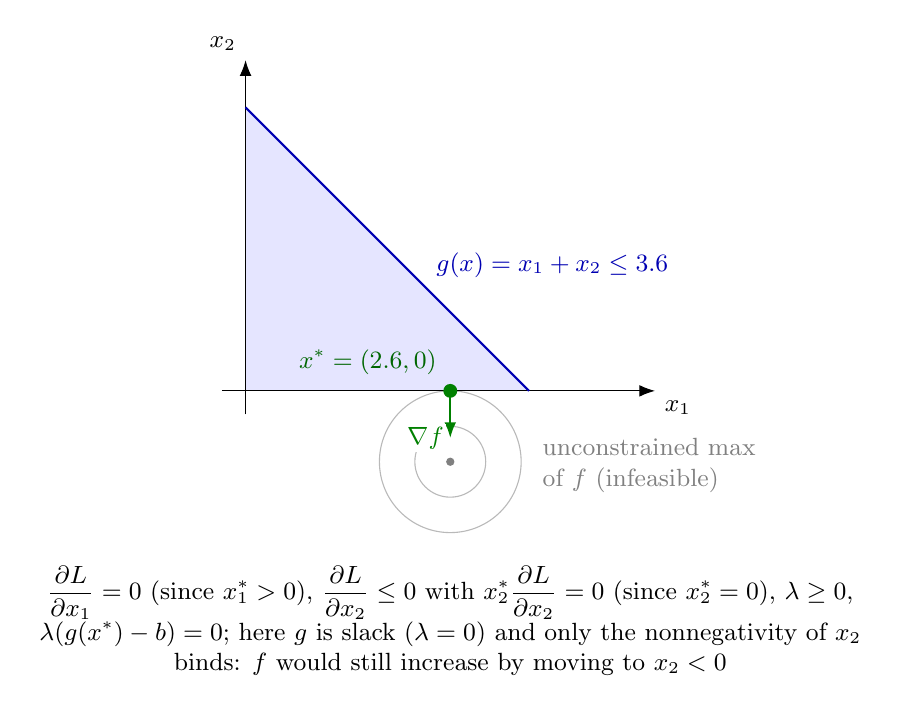
\begin{tikzpicture}[every node/.style={font=\small}, >={Latex[length=2mm]}, lab/.style={font=\small, fill=white, inner sep=1pt}]
	\fill[blue!10] (0,0) -- (3.6,0) -- (0,3.6) -- cycle;
	\foreach \r in {0.45,0.9} {\draw[gray!55] (2.6,-0.9) circle (\r);}
	\fill[gray] (2.6,-0.9) circle (1.5pt);
	\draw[->] (-0.3,0) -- (5.2,0) node[below right] {$x_1$};
	\draw[->] (0,-0.3) -- (0,4.2) node[above left] {$x_2$};
	\draw[blue!70!black, thick] (3.6,0) -- (0,3.6);
	\node[blue!70!black, font=\small, anchor=west] at (2.3,1.6) {$g(x)=x_1+x_2\le3.6$};
	\node[gray, font=\small, anchor=west, align=left] at (3.65,-0.95) {unconstrained max\\ of $f$ (infeasible)};
	\draw[->, green!50!black, thick] (2.6,0) -- (2.6,-0.6) node[left, lab, xshift=-1pt] {$\nabla f$};
	\fill[green!50!black] (2.6,0) circle (2.5pt);
	\node[green!40!black, anchor=south east, font=\small] at (2.55,0.08) {$x^\ast=(2.6,0)$};
	\node[anchor=north, align=flush center, text width=10.5cm] at (2.6,-2.1) {$\dfrac{\partial L}{\partial x_1}=0$ (since $x_1^\ast>0$), $\dfrac{\partial L}{\partial x_2}\le0$ with $x_2^\ast\dfrac{\partial L}{\partial x_2}=0$ (since $x_2^\ast=0$), $\lambda\ge0$, $\lambda(g(x^\ast)-b)=0$; here $g$ is slack ($\lambda=0$) and only the nonnegativity of $x_2$ binds: $f$ would still increase by moving to $x_2<0$};
\end{tikzpicture}
\end{document}
